\chapter{Part 5a. Multiprocessors Cache Coherence}
\textit{In the last chapter, we focused on how to get the most out of a single processor by exploring advanced parallelism techniques. Now, we’re moving to systems with multiple processors, where keeping their caches in sync is key to making everything work smoothly. This chapter introduces the basics of cache coherence and why it’s so important in shared-memory systems.}
\section{Flynn's Taxonomy (1966)}
Flynn's Taxonomy classifies computer architectures based on the number of instruction streams and data streams they support. It is divided into the following categories:
\begin{itemize}
    \item \textbf{SISD (Single Instruction, Single Data):} Represents uniprocessors where a single instruction stream operates on a single data stream. This is the traditional architecture of most early computers.

    \item \textbf{SIMD (Single Instruction, Multiple Data):} A single program executes on multiple data sets simultaneously. Classic examples include vector architectures used in high-performance computing, which are now less common. Modern x86 architectures support SIMD through various Instruction Set Architecture (ISA) extensions such as:
    \begin{itemize}
        \item MMX (1996)
        \item SSE (1999--2008)
        \item AVX (2011--2016)
    \end{itemize}

    \item \textbf{MIMD (Multiple Instruction, Multiple Data):} The general form of parallelism where each processor executes its own program on its own data. This is the most flexible and widely used parallel computing model.
\end{itemize}

\subsection{Shared-Memory Multiprocessors (UMA)}

Uniform Memory Access (UMA) is a shared-memory multiprocessor architecture where all processors have equal access time to the shared memory. This architecture is characterized by:
\begin{center}
    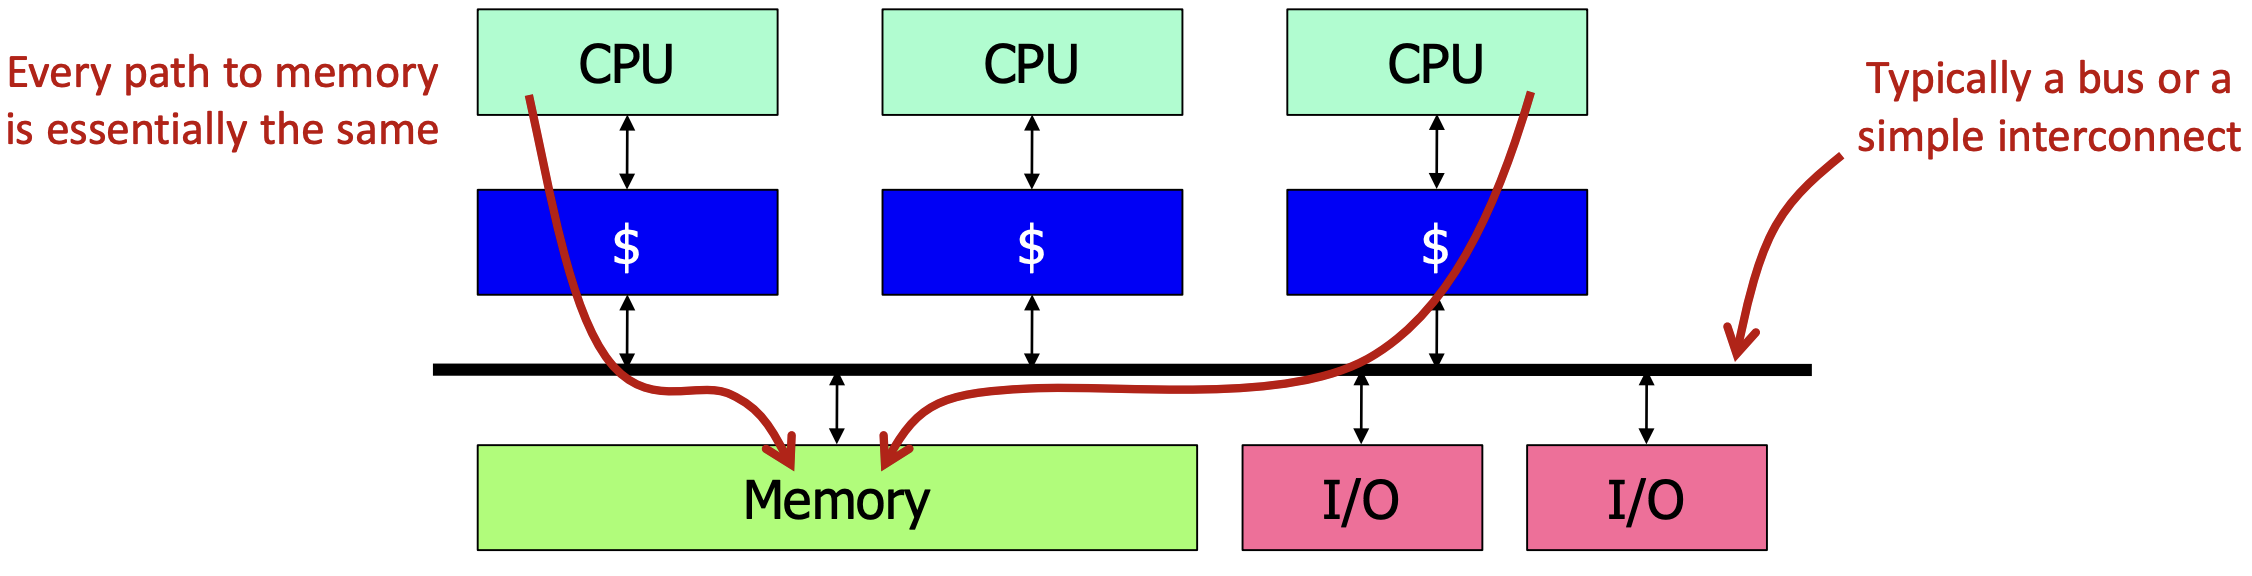
\includegraphics[width=0.65\textwidth]{chapters/chapter5a/images/smm.png}
\end{center}
\begin{itemize}
    \item \textbf{Uniform memory access:} Every path to memory is essentially the same, ensuring consistent performance across all processors.
    \item \textbf{Simple interconnect:} Typically, a bus or a basic interconnect is used to connect CPUs, caches, memory, and I/O devices.
    \item \textbf{Limited scalability:} UMA systems generally support 4 to 16 processors due to bottlenecks in the interconnect and memory access.
    \item \textbf{Traditional design:} UMA represents a simple and fairly traditional multiprocessor architecture suitable for small-scale parallel systems.
\end{itemize}

\subsection{Distributed-Memory Multiprocessors (NUMA)}
Nonuniform Memory Access (NUMA) is a distributed-memory multiprocessor architecture where each processor has its own local memory.
\begin{center}
    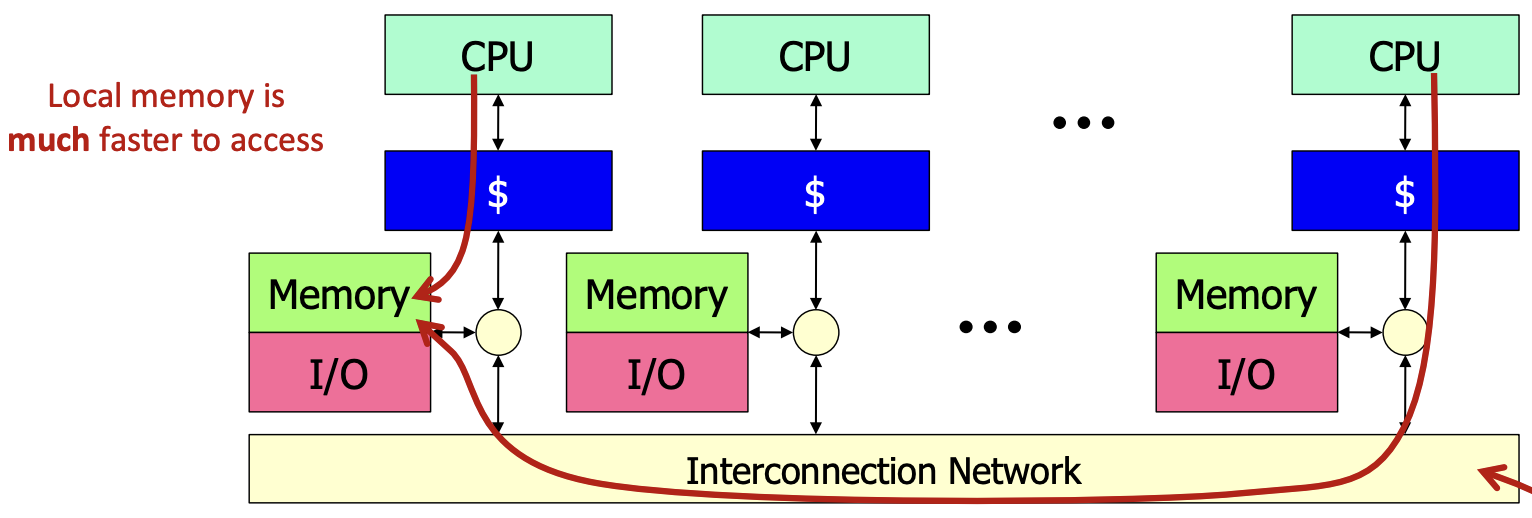
\includegraphics[width=0.65\textwidth]{chapters/chapter5a/images/dmm.png}
\end{center}
\begin{itemize}
    \item \textbf{Local memory access:} Each processor accesses its local memory much faster than the memory of other processors, leading to nonuniform memory access times.
    \item \textbf{Interconnection network:} Processors are connected through an interconnection network, which is often implemented as a real network, to enable communication and data exchange.
    \item \textbf{Scalability:} NUMA systems offer a more scalable and cost-effective way to grow the memory system, making them suitable for larger parallel systems.
    \item \textbf{Complex communication:} Communication between processors is more complex and involves higher latency compared to UMA systems.
\end{itemize}

\subsection{Programming Paradigms}
Parallel programming paradigms are classified based on how data is exchanged between processors. The two primary paradigms are:

\begin{itemize}
    \item \textbf{Shared-Memory:}
    \begin{itemize}
        \item Data is exchanged \emph{implicitly} through shared variables in a common memory space.
        \item Standard libraries (e.g., \texttt{OpenMP}) simplify programming.
        \item Well-suited for shared-memory architectures (e.g., SMP, NUMA).
        \item Can be implemented as \emph{Distributed Shared Memory (DSM)} on systems with physically distributed memory, using virtual memory abstractions (e.g., \texttt{TreadMarks} for DSM; \texttt{Apache Spark} for DSM-like abstractions in big data).
    \end{itemize}

    \item \textbf{Message Passing:}
    \begin{itemize}
        \item Data is exchanged \emph{explicitly} by sending and receiving messages over a network or interconnect.
        \item Standard libraries (e.g., \texttt{MPI}) are widely used.
        \item Natural for distributed-memory systems with private memory per processor.
        \item Can also be implemented on shared-memory systems (e.g., NUMA), although it may introduce unnecessary overhead compared to native shared-memory programming.
    \end{itemize}
\end{itemize}
\newpage
\subsection{Why (Hardware) Shared Memory?}

Shared memory provides a mechanism for parallel computing where multiple processors access a common memory space. Its advantages and disadvantages are as follows:

\begin{itemize}
    \item \textbf{Advantages:}
    \begin{itemize}
        \item Applications perceive it as a multitasking uniprocessor.
        \item Requires only evolutionary extensions for operating systems.
        \item Enables communication without relying on the operating system.
        \item Simplifies software development by allowing correctness to be prioritized over performance.
    \end{itemize}

    \item \textbf{Disadvantages:}
    \begin{itemize}
        \item Communication is implicit, making optimization more challenging.
        \item Synchronization between processors is complex.
        \item Places implementation demands on hardware designers.
    \end{itemize}

    \item \textbf{Result:}
    \begin{itemize}
        \item \emph{Symmetric Multiprocessors (SMPs):} Once the foundation of early supercomputers, SMPs have been largely replaced by distributed-memory message-passing systems due to scalability limitations.
        \item \emph{Chip Multiprocessors (CMPs) or Multicore Processors:} These dominate modern parallel computing, driving multibillion-dollar markets.
    \end{itemize}
\end{itemize}

\subsection{Cache Coherence and the Multi-Processor Problem}
\label{subsec:cache-coherence}

Cache coherence ensures that in a system with multiple processors,
all caches have a \emph{consistent} view of shared data. Without
coherence mechanisms, processors could read or write stale data in
their caches, leading to erroneous computation results.

\medskip

\noindent
\textbf{Example Scenario:}
\begin{center}
    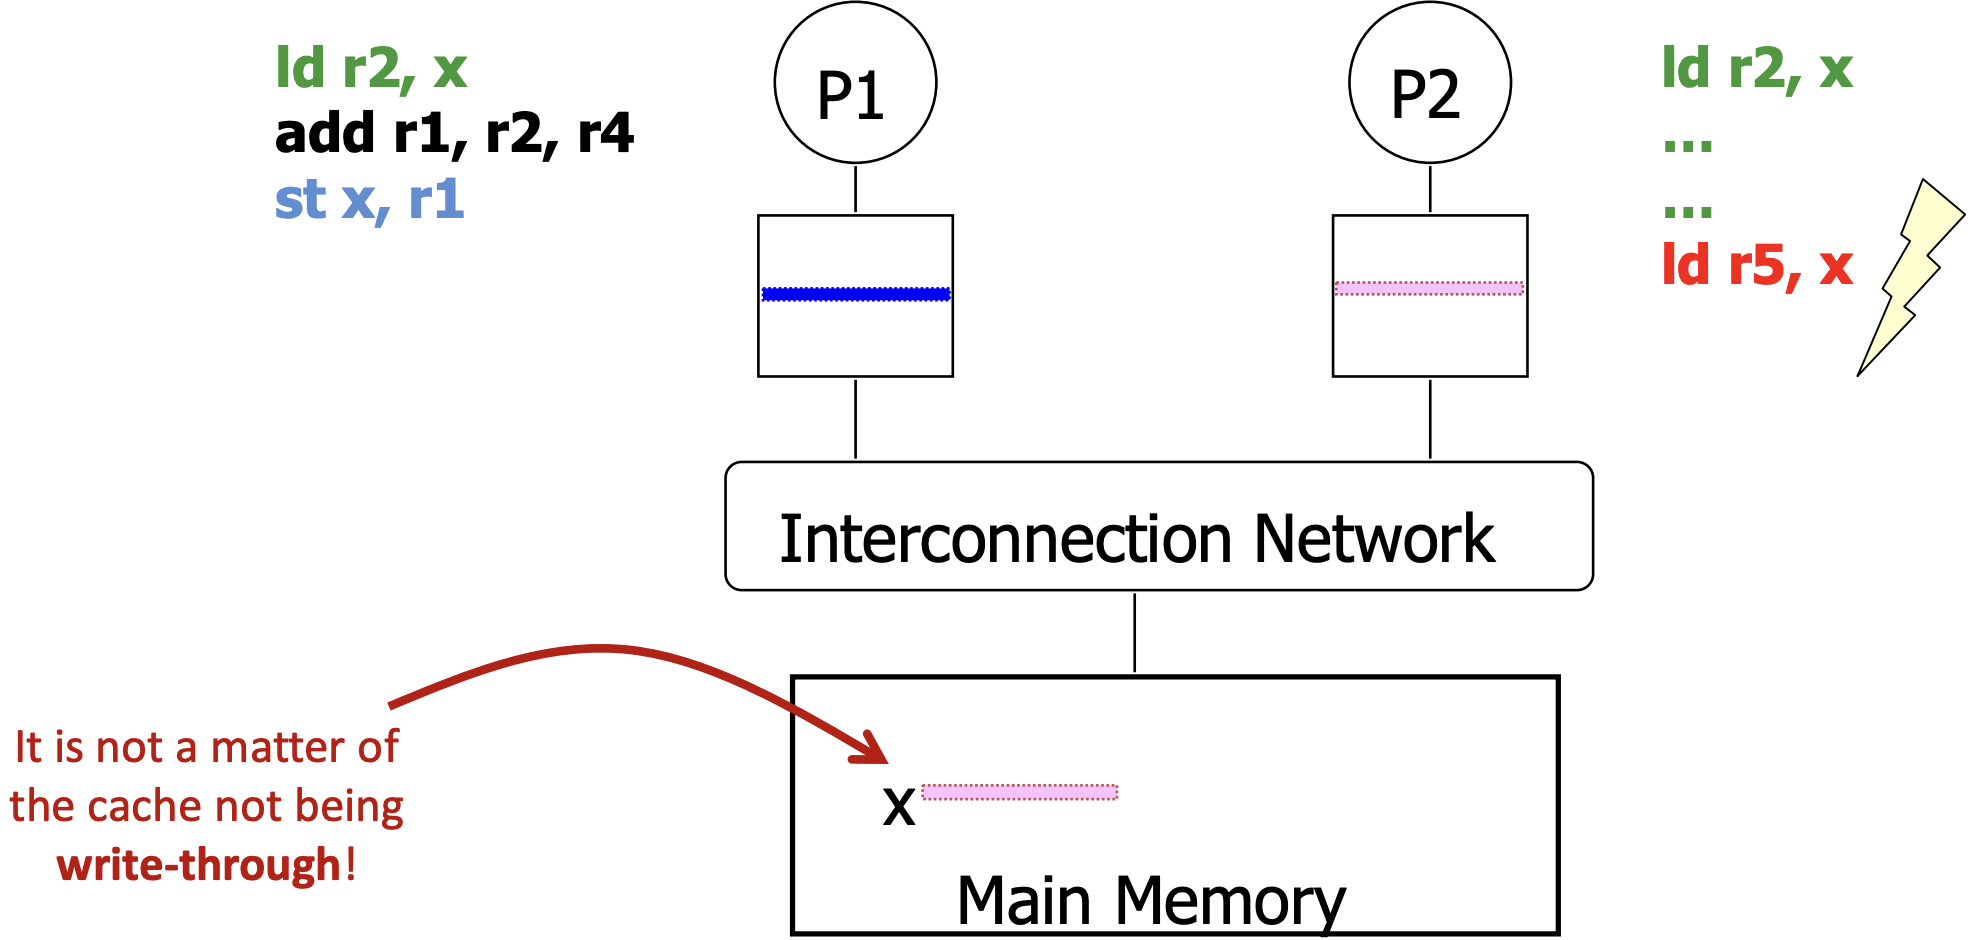
\includegraphics[width=0.55\textwidth]{chapters/chapter5a/images/incoherence.png}
\end{center}
\begin{enumerate}
  \item \textbf{Processor P1 loads a value:} Suppose a shared variable
  \texttt{x} in main memory holds an initial value. Processor~P1 loads
  \texttt{x} into its cache, so it now has a local copy of \texttt{x}.
  \item \textbf{Processor P2 also accesses \texttt{x}:} Later, P2 tries
  to read \texttt{x} but experiences a cache miss (since \texttt{x} is
  not yet in P2's cache). It fetches \texttt{x} from main memory, storing
  this same value in its own local cache.
  \item \textbf{P2 modifies \texttt{x}:} Processor~P2 then updates
  \texttt{x} directly in its cache (for instance, \texttt{st x, r1}).
  Depending on the cache write policy (\emph{write-back} vs.\
  \emph{write-through}), P2 may or may not immediately update main memory.
  \textbf{However, even if it does write to memory, P1's cache copy remains
  \emph{unchanged}.}
  \item \textbf{P1 sees stale data:} Because P1 already has a cached
  copy of \texttt{x}, it continues reading that older value (i.e.,
  the one loaded earlier).
\end{enumerate}

\medskip

\noindent
\textbf{Why is this a problem?}
The issue here is that multiple cached copies of the same data
must be kept in sync. If updates are performed in one cache without
informing other caches, the system can quickly become \emph{incoherent}.
A processor might base calculations on an incorrect, outdated value of
\texttt{x}, leading to unpredictable behavior or incorrect program
outputs.

\medskip

\noindent
\textbf{Importance of Coherence Protocols:}
To prevent such inconsistencies, cache coherence protocols enforce
invalidation or updating of stale cache lines. When one processor
modifies \texttt{x}, coherence messages are sent over the interconnection
network so that other caches either invalidate their copies or update
them with the new data. This ensures that all processors always see
a consistent view of shared memory.

\subsection{Ensuring a Coherent Memory System}
A \emph{coherent memory system} guarantees that every processor observes
all shared-memory operations (reads and writes) in a manner that is
logically consistent with a single, shared view of memory. The goals of
such a system typically boil down to the following three properties:

\begin{enumerate}
  \item \textbf{Preservation of program order.} If a processor $P$
  writes to a location \texttt{X} and then (without any intervening
  writes from other processors) reads \texttt{X}, it must read back the
  value that it just wrote. This ensures that each processor's own
  writes are visible to itself in program order.

  \item \textbf{Coherent view (read values).} If processor $P_1$ writes
  \texttt{X}, and processor $P_2$ then reads \texttt{X}$\!$, with no
  other intervening writes to \texttt{X}, $P_2$ must see the value
  written by $P_1$. Essentially, a read in one processor cannot observe
  an older version of \texttt{X}$\!$ if a newer version exists in the
  system and there have been no conflicting writes.

  \item \textbf{Write serialization.} If multiple processors write to
  \texttt{X} (e.g., $P_1$ writes, then $P_2$ writes, etc.), all
  processors must observe these writes in the same order. Thus, if $P_1$
  writes to \texttt{X}$\!$ first and $P_2$ writes to \texttt{X}$\!$
  second, then no processor should be able to observe $P_2$'s write
  before $P_1$'s write.
\end{enumerate}

\medskip

\noindent
\textbf{How do we achieve coherence in practice?}

\begin{itemize}
  \item \textbf{Hardware Protocols:} Coherence is typically enforced via
  specialized hardware protocols (e.g., MESI, MOESI) that track and
  coordinate the states of cache lines. When a processor writes to
  \texttt{X}, the protocol ensures other copies of \texttt{X} are either
  invalidated or updated.

  \item \textbf{Snooping or Directory-Based Approaches:} In
  \emph{snooping} protocols, all caches monitor a shared bus to detect
  writes and invalidate outdated copies. In \emph{directory-based}
  protocols, a central directory keeps track of which caches hold each
  line, allowing precise invalidation or update messages.

  \item \textbf{Preserving Order:} A coherence protocol enforces the
  three properties above by establishing rules for when a cache line
  can be read, written, invalidated, or shared. This ensures every
  processor eventually sees writes in the correct order and never
  operates on stale data.
\end{itemize}

\noindent
By carefully orchestrating which cache copy is valid and who has the
authority to write to it, a coherent memory system prevents the classic
inconsistencies shown in our earlier example. Processors remain
synchronized on shared data values, avoiding stale reads and enabling
correct parallel execution.


\subsection{Snoopy Cache-Coherence Protocols}
Snoopy cache-coherence protocols rely on a shared bus to serialize memory transactions and ensure data consistency across multiple caches. Each cache controller \emph{snoops} all bus transactions and compares them against the cache lines it currently holds. \\

\noindent \textbf{Basic Operation:}
\begin{itemize}
  \item \textbf{Bus as a Serialization Point:} All memory requests issued by processors appear on the shared bus, providing a single global ordering.
  \item \textbf{Snooping:} Each cache controller listens (\emph{snoops}) to every bus transaction. If a transaction concerns a cache line that the controller contains, it takes steps to maintain coherence.
\end{itemize}

\noindent \textbf{Coherence Actions:}
When a transaction targets a cache line, the responsible cache controller can:
\begin{itemize}
  \item \textit{Invalidate} a stale copy of the line.
  \item \textit{Update} its local line if another cache provides new data.
  \item \textit{Supply value} to another cache or to memory.
\end{itemize}
The specific action taken depends on the protocol’s finite state machine (FSM), which tracks the line’s state (e.g., \textit{Modified}, \textit{Shared}, \textit{Invalid}, etc.). \\
\smallskip
\noindent \textbf{Simultaneous Controllers:} \\
Each cache operates its snooping logic independently but concurrently. Because they all observe the same bus traffic, conflicts and updates are detected quickly, preserving coherence across the system. \\

This bus-based \emph{snoopy} approach is conceptually simpler than directory-based methods and is effective for a moderate number of processors sharing a single bus. However, as system scale increases, the performance overhead of snooping and bus contention may become a limiting factor.


\subsection{Simple Invalidate Snooping Protocol}
The Simple Invalidate Snooping Protocol is a cache coherence protocol designed for write-through, write-no-allocate caches. It operates with two states: \textbf{Valid} and \textbf{Invalid}. \\
Transitions between these states are governed by processor and bus actions.

\begin{center}
    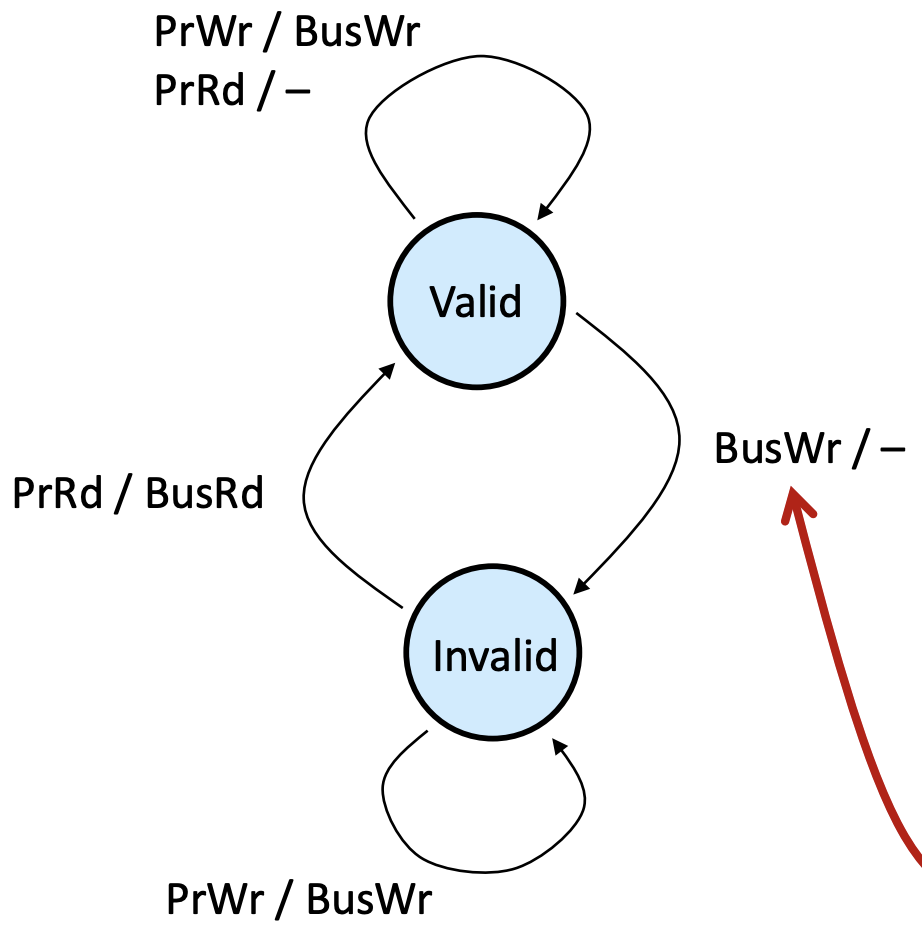
\includegraphics[width=0.3\textwidth]{chapters/chapter5a/images/basic.png}
\end{center}
\begin{itemize}
    \item[-] \textbf{Valid State}:
        \begin{itemize}
            \item A \texttt{PrWr} (Processor Write) results in a \texttt{BusWr} (Bus Write) operation.
            \item A \texttt{PrRd} (Processor Read) requires no bus action.
        \end{itemize}
    \item[-] \textbf{Invalid State}:
        \begin{itemize}
            \item A \texttt{PrRd} triggers a \texttt{BusRd} (Bus Read) to fetch data into the cache.
            \item A \texttt{PrWr} results in a \texttt{BusWr}.
        \end{itemize}
    \item[-] When another processor writes to the same cache line, a \texttt{BusWr} is broadcast, transitioning the state from \textbf{Valid} to \textbf{Invalid}.
    \item[-] A \texttt{BusRd} can transition the state from \textbf{Invalid} to \textbf{Valid}.
\end{itemize}

The protocol ensures coherence by invalidating or updating cache lines in response to snooped bus operations. This mechanism is essential in multiprocessor systems where caches are shared.

\textbf{Note:} The snooping mechanism actively monitors the bus to maintain coherence.

\subsection{3-State Write-Back Invalidation Protocol (MSI)}
The \textit{3-State Write-Back Invalidation Protocol (MSI)} is used to maintain cache coherence in multiprocessor systems. It introduces three states for cache lines:
\begin{itemize}
    \item \textbf{Modified (M):}
    \begin{itemize}
        \item The cache line contains the latest copy of the data.
        \item The memory is stale and not up-to-date.
        \item Only one cache can have this state for a given line.
    \end{itemize}

    \item \textbf{Shared (S):}
    \begin{itemize}
        \item The cache line contains a valid copy of the data.
        \item One or more caches may hold the same data in this state.
    \end{itemize}

    \item \textbf{Invalid (I):}
    \begin{itemize}
        \item The cache line is not valid and must be fetched from memory or another cache.
    \end{itemize}
\end{itemize}

\noindent\textbf{Features:}
\begin{itemize}
    \item Before entering the \textit{Modified} state, all other copies of the cache line must be invalidated.
    \item Ensures cache coherence by enforcing bus transactions to maintain order and perform invalidations.
\end{itemize}

\noindent\textbf{Comparison with 2-State Protocol:}
\begin{itemize}
    \item The 2-state protocol is simpler but less efficient, as every write operation requires a broadcast on the bus.
    \item MSI resolves coherence issues effectively, but it can lead to higher performance overhead due to bus transactions.
\end{itemize}

This protocol ensures coherence but can impact performance, particularly in systems with high contention for the memory bus.

\section{MSI Protocol}
%-----------------------------------------------------------------------
% Overview
%-----------------------------------------------------------------------
The \emph{Modified, Shared, Invalid} (MSI) protocol is a classic cache coherence protocol
used in multiprocessor systems with write-back caches. Its goal is to ensure that all
processors observe a consistent view of memory, even though multiple caches may hold
copies of the same memory block. In MSI, each cache block can be in exactly one of
three states at any time:

\begin{itemize}
  \item \textbf{M (Modified)}:
        The cache block holds the only valid (and most recent) copy of the data,
        and this copy has been modified with respect to main memory. Main memory
        is thus \emph{stale} until this block is written back.
  \item \textbf{S (Shared)}:
        One or more caches may contain valid copies of the data. The copy in main
        memory is also valid (i.e., the same as the cache blocks).
  \item \textbf{I (Invalid)}:
        The cache block is not valid. The data in this block must not be used
        without first fetching a valid copy from memory or another cache.
\end{itemize}

%-----------------------------------------------------------------------
% Diagram Placeholder
%-----------------------------------------------------------------------
\begin{center}
    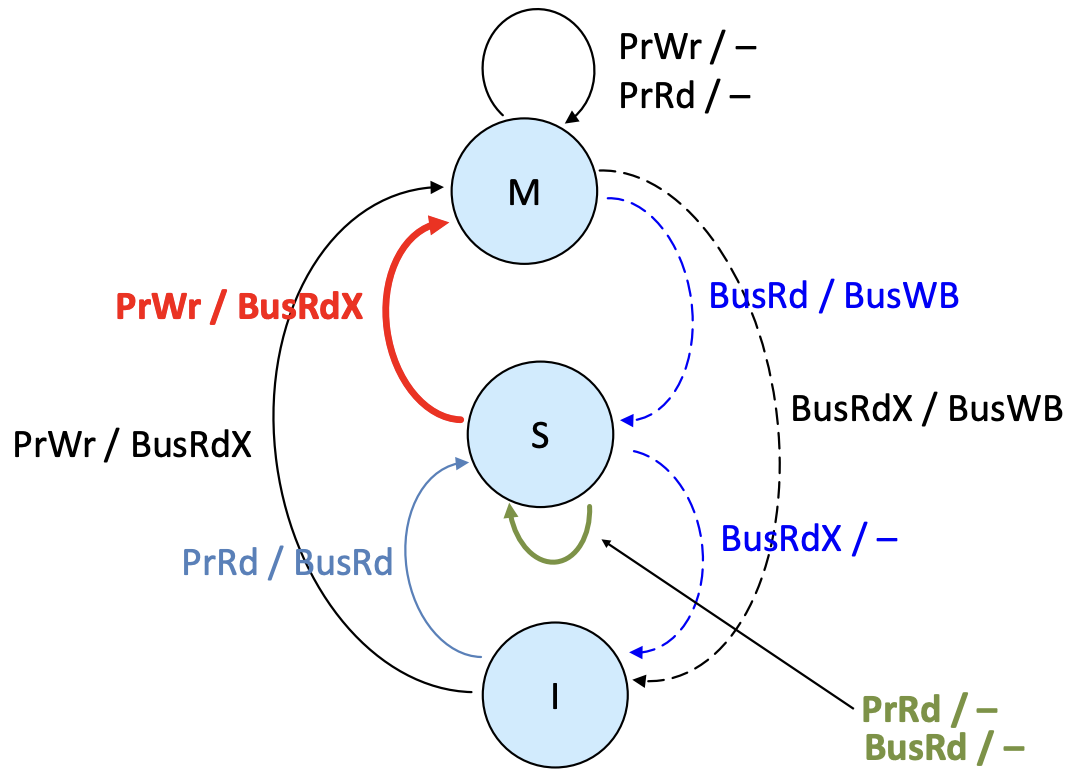
\includegraphics[width=0.55\textwidth]{chapters/chapter5a/images/msi.png}
\end{center}

%-----------------------------------------------------------------------
% States and Transitions Explanation
%-----------------------------------------------------------------------
The protocol enforces coherence by requiring certain \emph{bus transactions} on
reads and writes, which can cause cache blocks to transition from one state
to another. Typical bus signals include:
\begin{itemize}
  \item \textbf{BusRd (Bus Read)}: A read request \emph{without} intent to modify.
  \item \textbf{BusRdX (Bus Read Exclusive)}: A read request \emph{with} intent to modify
        (also called \emph{Read For Ownership}); it invalidates any other copies.
  \item \textbf{BusWB (Bus Write Back)}: A cache writes its modified block back to memory
        (or supplies it to another cache) when it must give up ownership.
\end{itemize}

Below is a concise description of the main state transitions (processor actions are
prefixed with \texttt{Pr} and bus actions with \texttt{Bus}):

\begin{itemize}
  \item \textbf{I $\rightarrow$ S}:
    Occurs on a \texttt{PrRd}, which triggers \texttt{BusRd} if the block is not present
    in any cache (or must be fetched from memory). The cache obtains a shared copy.
  \item \textbf{I $\rightarrow$ M}:
    Happens on a \texttt{PrWr}, leading to \texttt{BusRdX}. All other caches invalidate
    their copies before one cache transitions to Modified.
  \item \textbf{S $\rightarrow$ M}:
    On a \texttt{PrWr} to a shared block, the cache issues \texttt{BusRdX}, invalidating
    other shared copies and gaining exclusive (modified) ownership.
  \item \textbf{M $\rightarrow$ S}:
    If another processor performs a read (\texttt{BusRd}) while the block is in M,
    the current cache must supply the data via \texttt{BusWB}, and the block transitions
    to S (now shared among caches).
  \item \textbf{M or S $\rightarrow$ I}:
    An \texttt{Invalidate} request (triggered by someone else's \texttt{BusRdX}) or a
    coherence miss can force the local copy to become Invalid.
\end{itemize}

By following these rules, the MSI protocol ensures that at most one cache
holds a \textbf{Modified} copy and that any other copies are either \textbf{Shared} or
\textbf{Invalid}. This guarantees coherence across all caches and maintains
the illusion of a single, consistent memory.